% !TeX root=main.tex
\chapter{نتایج آزمایشات و ارزیابی عملکرد}
\section{مقدمه}

هدف این فصل ارزیابی معماری پیشنهادی از دو دیدگاه است: نخست، مدل نظری ظرفیت که بر اساس اندازه بلوک، فاصله بلوک و تعداد زنجیره‌های جانبی محاسبه می‌شود؛ دوم، بنچمارک\LTRfootnote{Benchmark} پیاده‌سازی به زبان راست\LTRfootnote{Rust} که ظرفیت محاسباتی نمونه اولیه را در محیط آزمایش نشان می‌دهد. تفکیک این دو دیدگاه ضروری است. عددی که در بنچمارک محاسباتی با دشواری پایین و بدون محدودیت واقعی شبکه به دست می‌آید، معادل توان عملیاتی یک شبکه عمومی واقعی نیست؛ بلکه نشان‌دهنده سقف پردازشی نرم‌افزار تحت شرایط کنترل‌شده است.

\section{محیط آزمایش}

پیاده‌سازی نمونه اولیه با زبان راست و در حالت انتشار بهینه‌شده\LTRfootnote{Release Mode} اجرا شده است. معیار اصلی اندازه‌گیری، زمان واقعی اجرا\LTRfootnote{Wall-clock Time} برای پردازش تعداد مشخصی تراکنش در پیکربندی‌های مختلف است. در نسخه فعلی، شبکه همتا‌به‌همتای کامل، تأخیر انتشار بلوک در اینترنت، رفتار خصمانه\LTRfootnote{Adversarial}، تأخیر جغرافیایی، و هزینه واقعی اعتبارسنجی امضا در مقیاس شبکه عمومی به طور کامل مدل نشده‌اند. بنابراین، نتایج آزمایش باید به عنوان ارزیابی نمونه اولیه و نه بنچمارک نهایی تولیدی تفسیر شود.

\begin{table}[h]
\centering
\caption{جدول ۴-۱. پارامترهای آزمایش}
\small
\begin{tabular}{|p{5.5cm}|p{8cm}|}
\hline
پارامتر & مقدار/توضیح \\
\hline
زبان پیاده‌سازی & راست \\
\hline
حالت اجرا & انتشار / بهینه‌شده \\
\hline
ساختار سیستم & زنجیره اصلی + \(N\) زنجیره جانبی \\
\hline
تعداد زنجیره‌های جانبی آزمایشی & ۱، ۲، ۳، ۵، ۱۰ \\
\hline
دشواری اثبات کار در آزمایش & پایین، برای اندازه‌گیری ظرفیت محاسباتی \\
\hline
معیار اصلی & تراکنش بر ثانیه، میانگین، میانه، حداقل، حداکثر، انحراف معیار \\
\hline
محدودیت شبکه واقعی & در این بنچمارک کامل اعمال نشده است \\
\hline
\end{tabular}
\end{table}

\section{مدل نظری شبکه}

با فرض بلوک یک مگابایتی و اندازه متوسط تراکنش ۲۵۰ بایت، تعداد تراکنش در هر بلوک حدود ۴۱۹۴ خواهد بود. اگر زنجیره اصلی هر ۶۰۰ ثانیه و زنجیره جانبی هر ۶۰ ثانیه بلوک تولید کند، داریم:

\begin{latin}
\[
TPS_{total} = 6.99 + 69.90N
\]
\end{latin}

\begin{figure}[h]
\centering
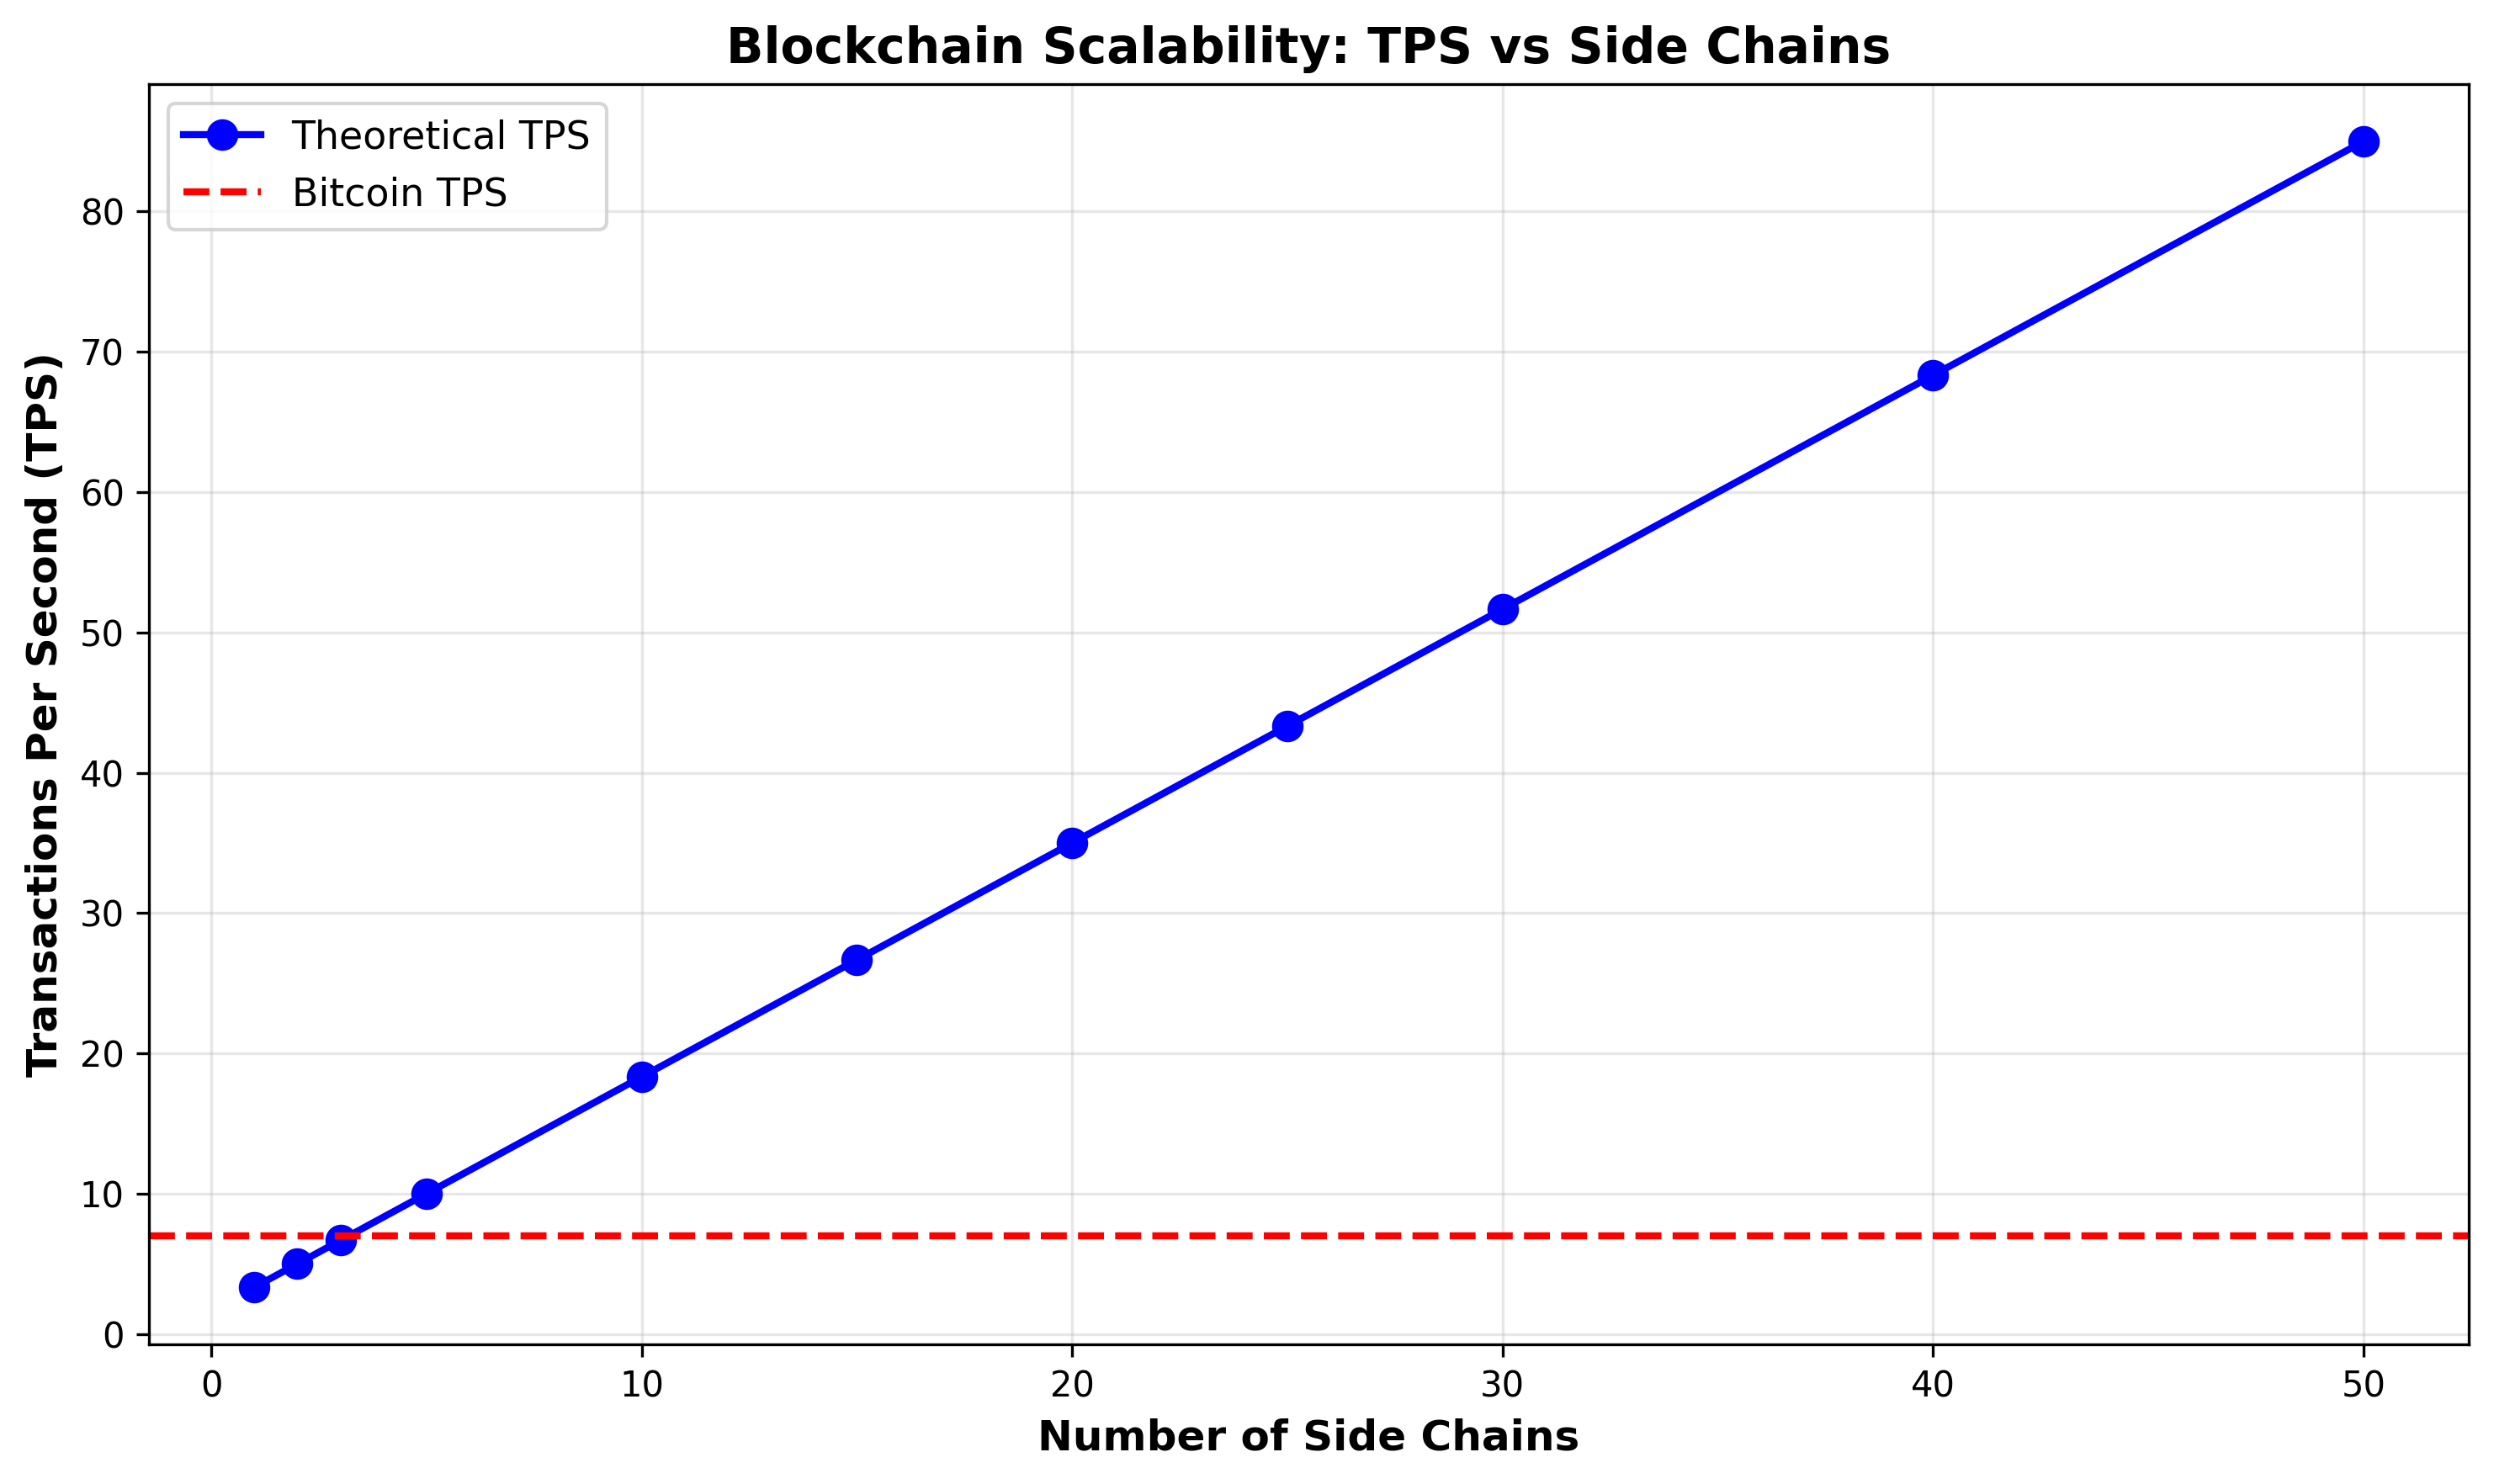
\includegraphics[width=0.92\linewidth]{img/tps_vs_sidechains.png}
\caption{مدل رشد خطی توان عملیاتی با تعداد زنجیره‌های جانبی}
\label{fig:tps-scalability}
\end{figure}


\begin{table}[h]
\centering
\caption{جدول ۴-۲. توان عملیاتی نظری با فرض بلوک یک مگابایتی و تراکنش ۲۵۰ بایتی}
\small
\begin{tabular}{|p{2.2cm}|p{2.8cm}|p{2.5cm}|p{2.8cm}|p{2.8cm}|}
\hline
تعداد زنجیره جانبی & توان زنجیره اصلی & توان زنجیره‌های جانبی & توان کل & بهبود نسبت به ۷ تراکنش بر ثانیه \\
\hline
۱ & ۶.۹۹ & ۶۹.۹۰ & ۷۶.۸۹ & ۱۱.۰ برابر \\
\hline
۳ & ۶.۹۹ & ۲۰۹.۷۰ & ۲۱۶.۶۹ & ۳۱.۰ برابر \\
\hline
۵ & ۶.۹۹ & ۳۴۹.۵۰ & ۳۵۶.۴۹ & ۵۰.۹ برابر \\
\hline
۱۰ & ۶.۹۹ & ۶۹۹.۰۰ & ۷۰۵.۹۹ & ۱۰۰.۹ برابر \\
\hline
۲۰ & ۶.۹۹ & ۱۳۹۸.۰۰ & ۱۴۰۴.۹۹ & ۲۰۰.۷ برابر \\
\hline
۵۰ & ۶.۹۹ & ۳۴۹۵.۰۰ & ۳۵۰۱.۹۹ & ۵۰۰.۳ برابر \\
\hline
۱۰۰ & ۶.۹۹ & ۶۹۹۰.۰۰ & ۶۹۹۶.۹۹ & ۹۹۹.۶ برابر \\
\hline
\end{tabular}
\end{table}

این جدول نشان می‌دهد که بهبود اصلی از تعداد زنجیره‌های جانبی می‌آید، نه صرفاً کوتاه‌تر کردن زمان بلوک. با یک زنجیره جانبی، ظرفیت حدود ۷۷ تراکنش بر ثانیه\LTRfootnote{Transactions Per Second (TPS)} است؛ با ۱۰۰ زنجیره جانبی، ظرفیت نظری به حدود ۷۰۰۰ تراکنش بر ثانیه می‌رسد.

\section{نتایج بنچمارک پیاده‌سازی}

نتایج بنچمارک نمونه اولیه در جدول زیر گزارش شده است.

\begin{table}[h]
\centering
\caption{جدول ۴-۳. نتایج بنچمارک محاسباتی پیاده‌سازی به زبان راست}
\small
\begin{tabular}{|p{1.4cm}|p{1.5cm}|p{1.5cm}|p{1.5cm}|p{1.5cm}|p{1.5cm}|p{1.6cm}|}
\hline
تعداد زنجیره جانبی & تعداد تراکنش آزمون & میانگین توان & میانه توان & حداقل توان & حداکثر توان & انحراف معیار \\
\hline
۱ & ۵۰ & ۴۴٬۸۲۴.۸۷ & ۴۵٬۰۶۸.۷۲ & ۳۹٬۲۳۲.۳۳ & ۵۰٬۱۷۳.۵۵ & ۵٬۴۷۴.۶۸ \\
\hline
۲ & ۱۰۰ & ۷٬۶۱۹.۸۹ & ۴٬۸۹۰.۹۹ & ۳٬۳۱۴.۷۱ & ۱۴٬۶۵۳.۹۸ & ۶٬۱۴۲.۴۷ \\
\hline
۳ & ۱۵۰ & ۷٬۰۴۹.۸۴ & ۷٬۱۱۳.۳۰ & ۵٬۰۸۵.۸۵ & ۸٬۹۵۰.۳۷ & ۱٬۹۳۳.۰۴ \\
\hline
۵ & ۲۵۰ & ۱۳٬۷۴۰.۷۰ & ۱۳٬۶۹۰.۸۸ & ۹٬۶۶۳.۱۱ & ۱۷٬۸۶۸.۱۰ & ۴٬۱۰۲.۷۲ \\
\hline
۱۰ & ۵۰۰ & ۸٬۹۳۴.۴۶ & ۱۰٬۱۱۷.۴۵ & ۶٬۱۴۴.۶۰ & ۱۰٬۵۴۱.۳۴ & ۲٬۴۲۵.۳۷ \\
\hline
\end{tabular}
\end{table}

این اعداد ظرفیت محاسباتی نمونه اولیه را نشان می‌دهند. مقدار بسیار بالای توان عملیاتی در حالت یک زنجیره جانبی به این دلیل است که محدودیت واقعی تولید بلوک، انتشار شبکه، اندازه بلوک و دشواری واقعی اثبات کار اعمال نشده است. همچنین، کاهش توان در برخی پیکربندی‌های چندزنجیره‌ای نشان می‌دهد سربار هماهنگی، مدیریت ساختارهای داده، تعویض زمینه پردازشی\LTRfootnote{Context Switching} و همزمانی می‌تواند اثر قابل توجهی داشته باشد.

\section{تحلیل تفاوت مدل نظری و بنچمارک}

وجود اختلاف میان مدل نظری شبکه و بنچمارک محاسباتی طبیعی است. مدل نظری بر محدودیت اندازه بلوک و فاصله بلوک مبتنی است. بنچمارک محاسباتی، زمان پردازش داخلی برنامه را اندازه می‌گیرد. بنابراین، اگر یک اجرای آزمایشی بتواند ده‌ها هزار تراکنش بر ثانیه پردازش کند، به این معنی نیست که شبکه عمومی با همان عدد نهایی می‌شود. شبکه واقعی با محدودیت‌های زیر روبه‌روست:

\begin{itemize}
\item انتشار بلوک میان نودهای جغرافیایی مختلف.
\item تأخیر شبکه و اتلاف بسته\LTRfootnote{Packet Loss}.
\item اعتبارسنجی امضاها و اسکریپت‌ها.
\item محدودیت اندازه بلوک و سیاست استخر تراکنش\LTRfootnote{Mempool}.
\item رقابت ماینرها و احتمال فورک\LTRfootnote{Fork}.
\item داده‌دسترسی بلوک‌های جانبی.
\item رفتار مهاجم و حملات منع سرویس\LTRfootnote{Denial of Service (DoS)}.
\end{itemize}

به همین دلیل، در سراسر این پایان‌نامه عددهایی مانند ۴۴٬۸۲۴ تراکنش بر ثانیه، «ظرفیت محاسباتی پیاده‌سازی در محیط کنترل‌شده» نامیده می‌شوند و نه توان عملیاتی شبکه واقعی؛ این دو کمیت از جنس متفاوتی هستند و خلط آن‌ها رایج‌ترین خطای گزارش‌دهی در کارهای مشابه است.

\section{مقایسه با راهکارهای موجود}

\begin{table}[h]
\centering
\caption{جدول ۴-۴. مقایسه کیفی معماری پیشنهادی با راهکارهای مقیاس‌پذیری}
\small
\begin{tabular}{|p{1.8cm}|p{1.6cm}|p{1.6cm}|p{1.6cm}|p{1.6cm}|p{1.8cm}|}
\hline
راهکار & مکانیزم & امنیت & پیچیدگی کاربر & رشد ظرفیت & محدودیت اصلی \\
\hline
بیتکوین پایه & لایه اول تک‌زنجیره‌ای & بسیار بالا & کم & ثابت & اندازه و زمان بلوک \\
\hline
افزایش اندازه بلوک & لایه اول بزرگ‌تر & بالا، با هزینه نود & کم & محدود & تمرکز نود \\
\hline
لایتنینگ & کانال پرداخت & وابسته به لایه اول و کانال & متوسط/بالا & وابسته به نقدینگی & مسیریابی و نقدینگی \\
\hline
رول‌آپ & اجرای برون‌زنجیره‌ای + اثبات/داده & نزدیک به لایه اول & متوسط & بالا & داده‌دسترسی و مرتب‌ساز \\
\hline
شاردینگ & تقسیم حالت/تراکنش & وابسته به شارد & پنهان از کاربر & خطی & امنیت شارد و تراکنش بین‌شاردی \\
\hline
زنجیره جانبی کلاسیک & زنجیره مستقل & وابسته به پل/اجماع & متوسط & متغیر & مدل اعتماد \\
\hline
معماری پیشنهادی & چند زنجیره جانبی + زنجیره اصلی & امنیت نهایی از زنجیره اصلی & متوسط & تقریباً خطی با \(N\) & تراکنش بین‌زنجیره‌ای و هماهنگی \\
\hline
\end{tabular}
\end{table}

\section{تحلیل حساسیت}

برای تحلیل حساسیت، می‌توان اثر سه پارامتر اصلی را بررسی کرد: تعداد زنجیره‌های جانبی، اندازه بلوک و فاصله بلوک جانبی. طبق مدل:

\begin{latin}
\[
TPS = \frac{M}{T_m} + \frac{NS}{T_s}
\]
\end{latin}

افزایش \(N\) اثر خطی دارد. افزایش \(S\)، که معمولاً تابع اندازه بلوک است، نیز اثر خطی دارد، اما هزینه نود را افزایش می‌دهد. کاهش \(T_s\) ظرفیت را افزایش می‌دهد، اما احتمال فورک و فشار انتشار را بالا می‌برد. بنابراین، انتخاب پارامترها باید با توجه به هدف سامانه انجام شود. برای یک شبکه عمومی، محافظه‌کاری در \(T_s\) و \(S\) ضروری است؛ اما در یک شبکه سازمانی یا مجوزدار\LTRfootnote{Permissioned}، می‌توان پارامترها را تهاجمی‌تر انتخاب کرد.

\section{تهدیدهای اعتبار ارزیابی}

اعتبار نتایج این پایان‌نامه از چند جهت محدود است:

\begin{itemize}
\item \textbf{اعتبار داخلی:} ممکن است اندازه نمونه تراکنش‌ها، دشواری پایین یا ساختار داده‌های ساده باعث افزایش مصنوعی توان اندازه‌گیری‌شده شده باشد.
\item \textbf{اعتبار خارجی:} نتایج روی یک محیط آزمایشی الزاماً به شبکه جهانی با هزاران نود تعمیم‌پذیر نیست.
\item \textbf{اعتبار سازه‌ای:} توان عملیاتی به تنهایی معیار کامل نیست و باید تأخیر، قطعیت نهایی، نرخ فورک و هزینه نود نیز بررسی شود.
\item \textbf{اعتبار بازتولید:} برای بازتولید، باید نسخه کد، سخت‌افزار، سیستم‌عامل، پارامترها و روش اجرای بنچمارک ثبت شود.
\end{itemize}

\section{پیشنهاد پروتکل ارزیابی کامل‌تر}

برای ارزیابی دقیق‌تر در آینده، پیشنهاد می‌شود آزمایش‌ها در چهار سطح انجام شوند:

\begin{enumerate}
\item \textbf{آزمایش واحد:} اعتبارسنجی تراکنش، خروجی‌های خرج‌نشده، هش و امضا.
\item \textbf{آزمایش محلی:} اجرای چند زنجیره روی یک ماشین برای سنجش سربار نرم‌افزاری.
\item \textbf{آزمایش شبکه کنترل‌شده:} اجرای نودها روی چند ماشین یا کانتینر با تأخیر مصنوعی.
\item \textbf{آزمایش خصمانه:} شبیه‌سازی حملات دوبارخرج، تأخیر انتشار، فورک و سانسور.
\end{enumerate}

همچنین بهتر است برای هر پیکربندی حداقل ۳۰ تکرار انجام شود و علاوه بر میانگین، فاصله اطمینان و نمودار توزیع گزارش گردد.

\section{تحلیل حذف اجزا}

برای اینکه سهم هر جزء معماری روشن شود، انجام مطالعه حذف اجزا\LTRfootnote{Ablation Study} ضروری است. در این نوع مطالعه، هر بار یکی از اجزای معماری حذف یا ساده‌سازی می‌شود و اثر آن بر عملکرد و امنیت اندازه‌گیری می‌گردد. برای این پایان‌نامه، چند آزمایش حذف مهم پیشنهاد می‌شود:

\begin{itemize}
\item اجرای سیستم با یک زنجیره جانبی در برابر چند زنجیره جانبی، برای سنجش اثر موازی‌سازی.
\item حذف ثبت ارجاع در زنجیره اصلی، برای نشان دادن نقش لنگر امنیتی.
\item اجرای تابع تخصیص تصادفی در برابر تابع تخصیص مبتنی بر خروجی‌های خرج‌نشده، برای سنجش اثر سازگاری و دوبارخرج.
\item افزایش تدریجی دشواری اثبات کار جانبی، برای بررسی رابطه امنیت و توان عملیاتی.
\item فعال و غیرفعال کردن تراکنش بین‌زنجیره‌ای، برای سنجش سربار بین‌زنجیره‌ای.
\end{itemize}

از میان این پنج مورد، تنها مورد نخست در بنچمارک فعلی پوشش داده شده است (جدول ۴-۳ عملاً مقایسه یک زنجیره با چند زنجیره است). چهار مورد دیگر به تغییراتی در کد نمونه اولیه نیاز دارند ــ به‌ویژه امکان خاموش کردن ثبت ارجاع و تزریق تراکنش بین‌زنجیره‌ای با نرخ قابل تنظیم ــ و به همین دلیل به عنوان طرح آزمایش برای ادامه کار مشخص شده‌اند. انتظار ما این است که آزمایش دوم (حذف ارجاع) اثر محسوسی بر توان عملیاتی نداشته باشد اما مدل امنیتی را عوض کند، و آزمایش پنجم (فعال کردن تراکنش بین‌زنجیره‌ای) با افزایش سهم تراکنش‌های متقاطع، انحراف از رشد خطی را به شکل قابل اندازه‌گیری نشان دهد.

\section{تحلیل خطا و موارد شکست}

هر سامانه مقیاس‌پذیر باید موارد شکست خود را بشناسد. در معماری پیشنهادی، چند حالت شکست\LTRfootnote{Failure Case} مهم وجود دارد. نخست، اگر یک زنجیره جانبی بسیار شلوغ شود، تأخیر آن بالا می‌رود در حالی که زنجیره‌های دیگر ممکن است خلوت باشند. دوم، اگر ماینرهای یک زنجیره جانبی تبانی کنند، می‌توانند برای مدت کوتاه تراکنش‌ها را سانسور یا فورک ایجاد کنند. سوم، اگر داده بلوک جانبی منتشر نشود، ارجاع ثبت‌شده در زنجیره اصلی از نظر عملی قابل اعتبارسنجی نیست. چهارم، اگر تراکنش بین‌زنجیره‌ای در میانه مسیر متوقف شود، دارایی ممکن است تا زمان مهلت زمانی قفل بماند. پنجم، اگر تعداد زنجیره‌ها بدون سیاست دوره‌بندی تغییر کند، اختلاف در تابع تخصیص رخ می‌دهد.

تحلیل این خطاها دو فایده دارد. از یک سو، نشان می‌دهد معماری پیشنهادی نسبت به محدودیت‌های خود آگاه است. از سوی دیگر، مسیرهای دقیق بهبود را مشخص می‌کند. برای مثال، مشکل داده‌دسترسی با الزام انتشار داده و اثبات مرکل کاهش می‌یابد؛ مشکل امنیت زنجیره جانبی با استخراج ادغام‌شده\LTRfootnote{Merged Mining} یا ایست‌گذاری سریع‌تر قابل کاهش است؛ مشکل عدم تعادل بار با کارمزد پویا و مهاجرت قابل مدیریت است.

\section{تحلیل هزینه اجرای نود}

افزایش توان عملیاتی اگر باعث شود فقط چند نود قدرتمند توان اجرای شبکه را داشته باشند، با هدف غیرمتمرکز بودن ناسازگار است. بنابراین، باید هزینه اجرای نود بررسی شود. در معماری پیشنهادی، سه نوع نود قابل تعریف است:

\begin{itemize}
\item نود کامل اصلی: فقط زنجیره اصلی و ارجاعات را نگهداری می‌کند.
\item نود کامل جانبی: یک یا چند زنجیره جانبی را اعتبارسنجی می‌کند.
\item نود آرشیوی کامل: زنجیره اصلی و همه زنجیره‌های جانبی را نگهداری می‌کند.
\end{itemize}

این تفکیک به کاربران اجازه می‌دهد بسته به نیاز خود سطح مشارکت را انتخاب کنند. با این حال، اگر تعداد زیادی از کاربران فقط نود اصلی سبک اجرا کنند و تعداد نودهای جانبی کم باشد، امنیت عملی زنجیره‌های جانبی کاهش می‌یابد. بنابراین، در طراحی نهایی باید حداقل تعداد نود جانبی، سیاست پاداش و ابزارهای ساده اجرای نود در نظر گرفته شود.

\section{تحلیل اقتصادی ساده}

افزایش ظرفیت معمولاً باعث کاهش رقابت برای فضای بلوک و در نتیجه کاهش کارمزد متوسط می‌شود. اگر ظرفیت جانبی زیاد باشد، کاربران برای تراکنش‌های عادی می‌توانند کارمزد کمتر پرداخت کنند. اما از سوی دیگر، امنیت زنجیره‌های جانبی نیازمند پاداش کافی برای ماینرها یا اعتبارسنج‌هاست. بنابراین، کارمزد نباید آن‌قدر پایین باشد که انگیزه مشارکت از بین برود.

یک مدل ساده هزینه تراکنش چنین است:

\begin{latin}
\[
Cost_{tx} = Fee_{side} + Fee_{anchor}/BatchSize
\]
\end{latin}

در این فرمول، کاربر کارمزد جانبی را برای پردازش تراکنش و سهمی از کارمزد ثبت ارجاع را پرداخت می‌کند. هرچه تعداد تراکنش‌های یک بلوک جانبی بیشتر باشد، هزینه سرشکن‌شده ثبت ارجاع کمتر می‌شود. این ویژگی یکی از مزایای دسته‌بندی ارجاعات است.

\section{جمع‌بندی فصل}

نتایج این فصل از دو جنس بودند و باید از هم تفکیک شوند. مدل نظری نشان داد که با فرض توزیع متعادل بار و کافی بودن ظرفیت ارجاع در زنجیره اصلی، ظرفیت کل با تعداد زنجیره‌های جانبی رشد خطی دارد و با صد زنجیره جانبی به مرتبه چند هزار تراکنش بر ثانیه می‌رسد. بنچمارک پیاده‌سازی به زبان راست نیز نشان داد هسته پردازشی نمونه اولیه سریع است، اما همان نتایج، سربار هماهنگی چندزنجیره‌ای روی یک ماشین را هم آشکار کردند: در برخی پیکربندی‌ها افزودن زنجیره، به دلیل رقابت بر سر منابع مشترک، توان اندازه‌گیری‌شده را کاهش داد. این مشاهده به خودی خود یافته مفیدی است، چون نشان می‌دهد رشد خطی نظری فقط وقتی محقق می‌شود که منابع پردازشی نیز همراه با زنجیره‌ها افزوده شوند.

در کنار اعداد، این فصل چارچوب ارزیابی را نیز صریح کرد: تمایز ظرفیت محاسباتی از توان شبکه واقعی، فهرست تهدیدهای اعتبار، طرح مطالعه حذف اجزا، تحلیل موارد شکست و هزینه اجرای نود. نتیجه کلی آن است که معماری پیشنهادی پتانسیل مقیاس‌پذیری ساختاری دارد، اما اثبات کارایی تولیدی آن به آزمایش شبکه‌ای توزیع‌شده، تحلیل امنیتی عمیق‌تر و تکمیل پروتکل داده‌دسترسی گره خورده است؛ سه موضوعی که فصل بعد آن‌ها را در قالب کارهای آینده جمع‌بندی می‌کند.
